\documentclass[11pt]{beamer}
\usetheme{CambridgeUS}
\usepackage[utf8]{inputenc}
\usepackage[german]{babel}
\usepackage{amsmath}
\usepackage{amsfonts}
\usepackage{amssymb}
\usepackage{url}
%\pgfpageuselayout{4 0n 1 with notes}[a4paper,border shrink=5mm]
\usepackage{color}
\definecolor{mygreen}{rgb}{0,0.6,0}
\definecolor{mygray}{rgb}{0.5,0.5,0.5}
\usepackage{listings}
% https://en.wikibooks.org/wiki/LaTeX/Source_Code_Listings
\lstset{basicstyle=\scriptsize % http://texblog.org/2012/08/29/changing-the-font-size-in-latex/
        , commentstyle=\color{mygreen}
        , keywordstyle=\color{blue}
        , language=C++
        %, frame=single
    }

\author{Richard Ulrich}
\title{Trustworthy Software}
\subtitle{Why we sign our binaries and installers}
\setbeamercovered{dynamic} 
\institute{BORM Informatik AG} 
%\date{} 
\subject{BORM developer day} 
\titlegraphic{
\includegraphics[width=2cm]{borm_logo.jpg}}

\begin{document}

\begin{frame}
\titlepage
\end{frame}

%\begin{frame}
%\tableofcontents
%\end{frame}

\begin{frame}{warning when installing PointLine}
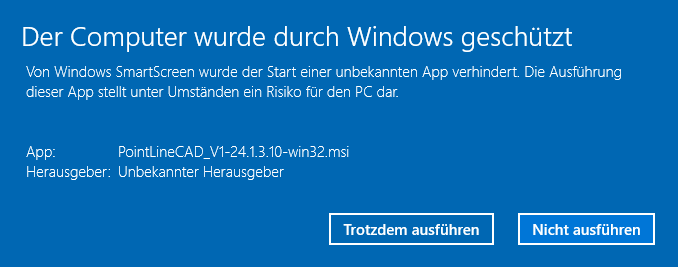
\includegraphics[scale=0.5]{obsolete_signature.png}
% some of you might have noticed for the first time that we sign our installers
% when this warning started appearing at the start of 2016 upon trying to 
% install PointLine
\end{frame}

\begin{frame}{PointLine signature}
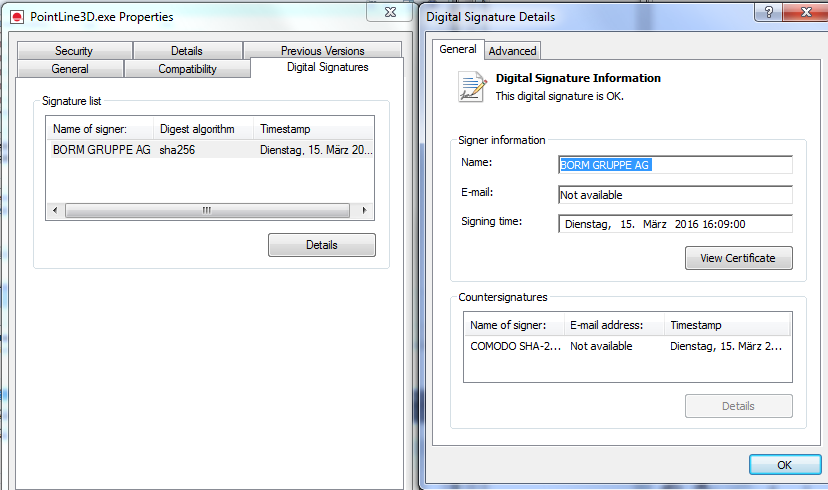
\includegraphics[scale=0.38]{pointLine_signature.png}
% you can inspect the signature yourself by right-clicking a program file or dll
% The important part is : "This digital signature is OK."
\end{frame}

\begin{frame}{How code signing works}
\emph{Pre-conditions}
\begin{itemize}
\item Create a large random private key
\item The public key is derived from it
\item Buy a certificate for your public key
\end{itemize}
\pause
\\[0.2cm]
\emph{Signing the software}
\begin{itemize}
\item Create a digest (hash) of the binary
\item Sign it with the private key
\item Public key and certificate are attached to the signed binary
\end{itemize}
\pause
\\[0.2cm]
\emph{Verifying the signature}
\begin{itemize}
\item Everybody with the public key can verify the signature
\item Certificate creates trust link to known root
\item Roots are shipped with the operating system
\end{itemize}
% most of this also applies to tls certificates for secure web browsing
\end{frame}

\begin{frame}{What the signature asserts}
\begin{itemize}
\item Publisher assures that the software is genuine
\item The file did not change since it was signed
\item It was signed on the indicated day (timestamp)
\end{itemize}
\end{frame}

\begin{frame}{How do we know the signature is from whom it says}
\begin{itemize}
\item Borm bought a certificate from a certificate authority.
\item The certificate authority checked a trade register document.
\item The certificate authority bought a certificate from a root authority.
\item Root certificates are shipped with the operating system
\end{itemize}
\end{frame}

\begin{frame}{certificate authority hierarchies}
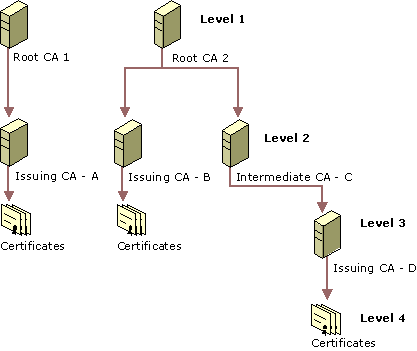
\includegraphics[scale=0.5]{certificate_authority_hierarchies.png}
% source : https://technet.microsoft.com/en-us/library/cc962065.aspx
\end{frame}

\begin{frame}{What attacks does the signature protect against}
\begin{itemize}
\item Tampering with the licensing mechanism and selling as original
\item Tampering with the software to make it buggy
\item Bundling malware by copycat publisher (angry bird clones)
\item Bundling malware by proxy or man in the middle (ISP, public WiFi, tor exit nodes, great firewall of china)
\item Bundling malware by download site (sourceforge)
\end{itemize}
\end{frame}

\begin{frame}{definition of malware}
\emph{Malware}, short for malicious software, is any software used to disrupt computer operations, gather sensitive information, gain access to private computer systems, or display unwanted advertising.
\\[0.2cm]
Malware is defined by its malicious intent, acting against the requirements of the computer user, and does not include software that causes unintentional harm due to some deficiency.
\\[0.2cm]
source: \href{https://en.wikipedia.org/wiki/Malware}{https://en.wikipedia.org/wiki/Malware}
% the border between malware and crapware is not always clear
\end{frame}

\begin{frame}{definition of backdoor}
A backdoor is a method, often secret, of bypassing normal authentication in a product, computer system, cryptosystem or algorithm etc.
\\[0.2cm]
Backdoors are often used for securing unauthorized remote access to a computer, or obtaining access to plaintext in cryptographic systems.
\\[0.2cm]
source: \href{https://en.wikipedia.org/wiki/Backdoor\textunderscore(computing)}{https://en.wikipedia.org/wiki/Backdoor\_(computing)}
\end{frame}

\begin{frame}{ISP's injecting malware}
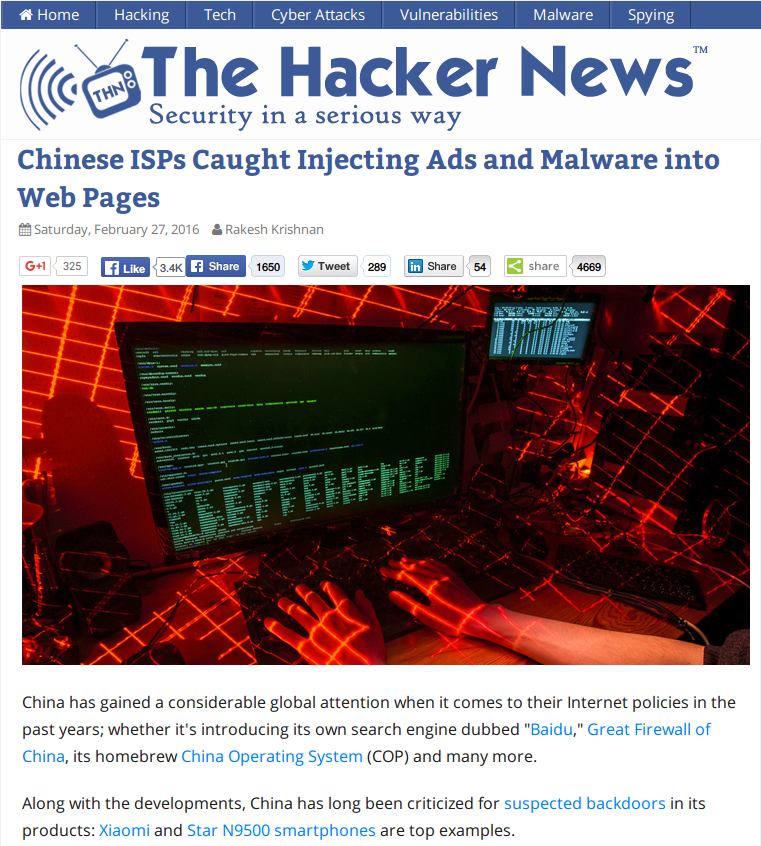
\includegraphics[scale=0.28]{isp_malware.png}
\end{frame}

\begin{frame}{tor exit node tamper windows update}
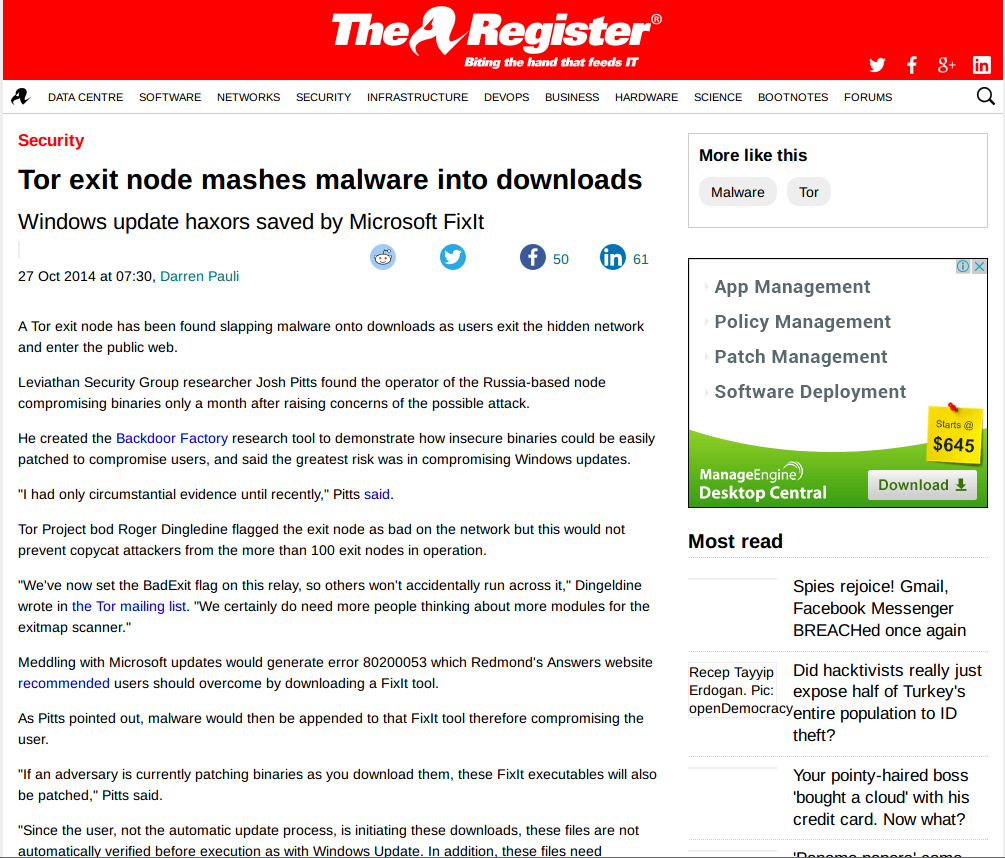
\includegraphics[scale=0.3]{tor_exit_windows_update.png}
\end{frame}

\begin{frame}{injecting js for ddos}
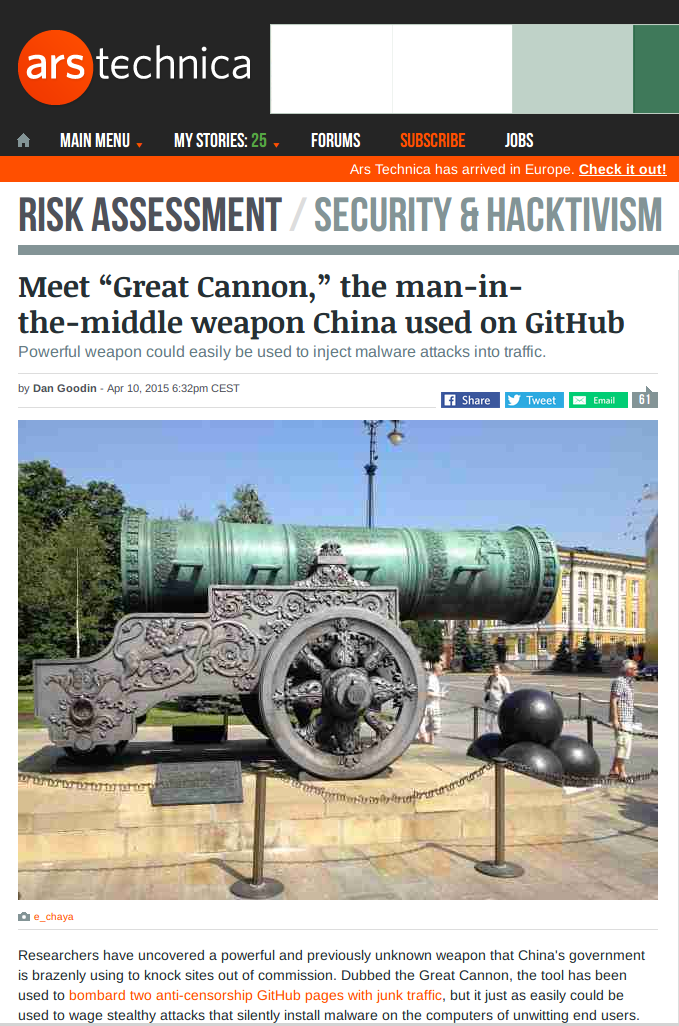
\includegraphics[scale=0.2]{great_canon.png}
%http://arstechnica.com/security/2015/04/meet-great-cannon-the-man-in-the-middle-weapon-china-used-on-github/
\end{frame}

\begin{frame}{What attacks does code signing not protect against}
\begin{itemize}
\item Weak hash or crypto used for the signature            % we only recently switched to SHA256 hash
\item Hacker sneaking backdoors into source code            % sane version control is a protection
\item Coerced employee sneaking backdoors into source code  % good code reviews are a protection
\item Publisher intentionally adding backdoors              % skype story later
\item Compromised build environment (computer)              % very serious
\item Compromised build tools (compiler)                    % very serious
\item Bundling malware by publisher (oracle java)
\item Insecure coding practices
\item Bribed timestamping provider                          % the least serious
\item Compromised certificate authority
\item Private key stolen or unintentionally published
\end{itemize}
% how could we fix these problems?
% let's look at them one at a time.
\end{frame}

\begin{frame}{Weak hash or crypto used for the signature}
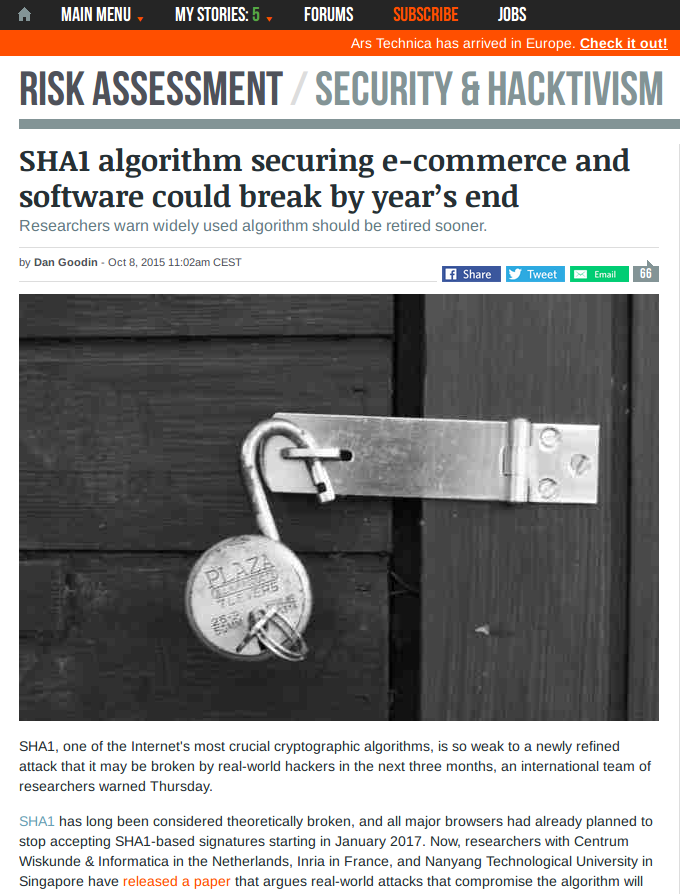
\includegraphics[scale=0.27]{sha1.png}
% This is what triggered the warning on the first slide
% It was relatively easy to fix
% We bought a new certificate and adapted the build process
\end{frame}

\begin{frame}{Backdoors in the source code}
\emph{Developers can mitigate the risk using:}
\begin{itemize}
\item Good version control system
\item Code reviews
\item Having control over artefacts % tampering with 3rd party libs might be harder to detect
\end{itemize}
\\[0.2cm]
\pause
\emph{But how can the user be confident enough?}
\begin{itemize}
\item Reputation                    % not enough, but ofthen that's all you get
\item Promises                      % really?
\item Independent code reviews      % doesn't fit well with agile development
\item OpenSource                    % convincing - the only way you can really trust your software
\end{itemize}
\end{frame}

\begin{frame}{skype backdoor}
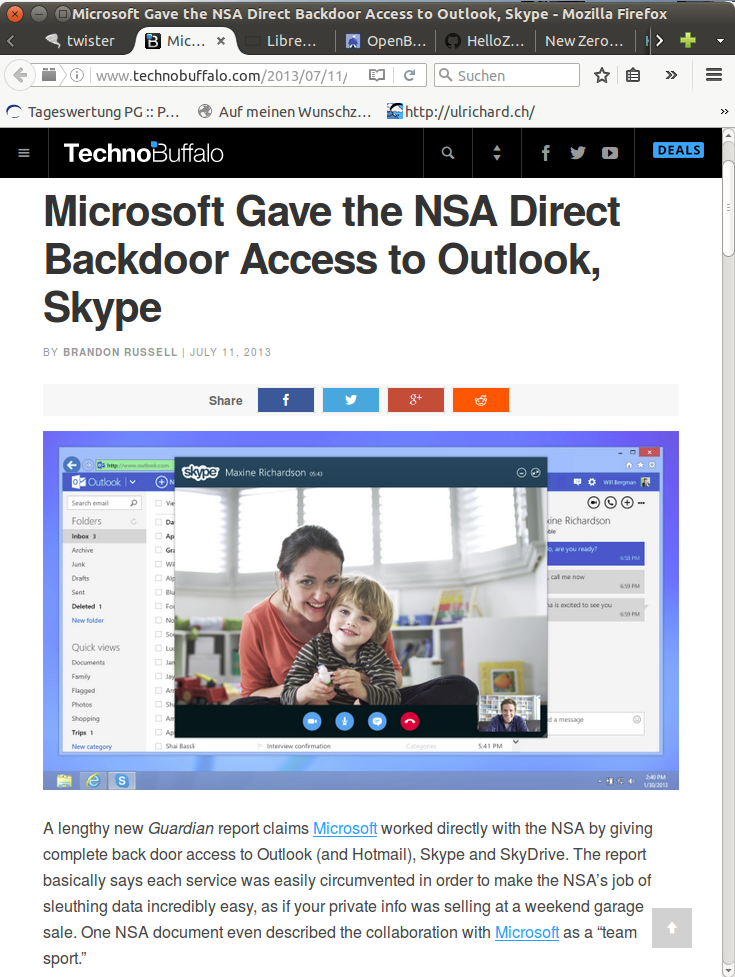
\includegraphics[scale=0.27]{skype.png}
% no big surprise from that company
\end{frame}

\begin{frame}{backdoors for criminals}
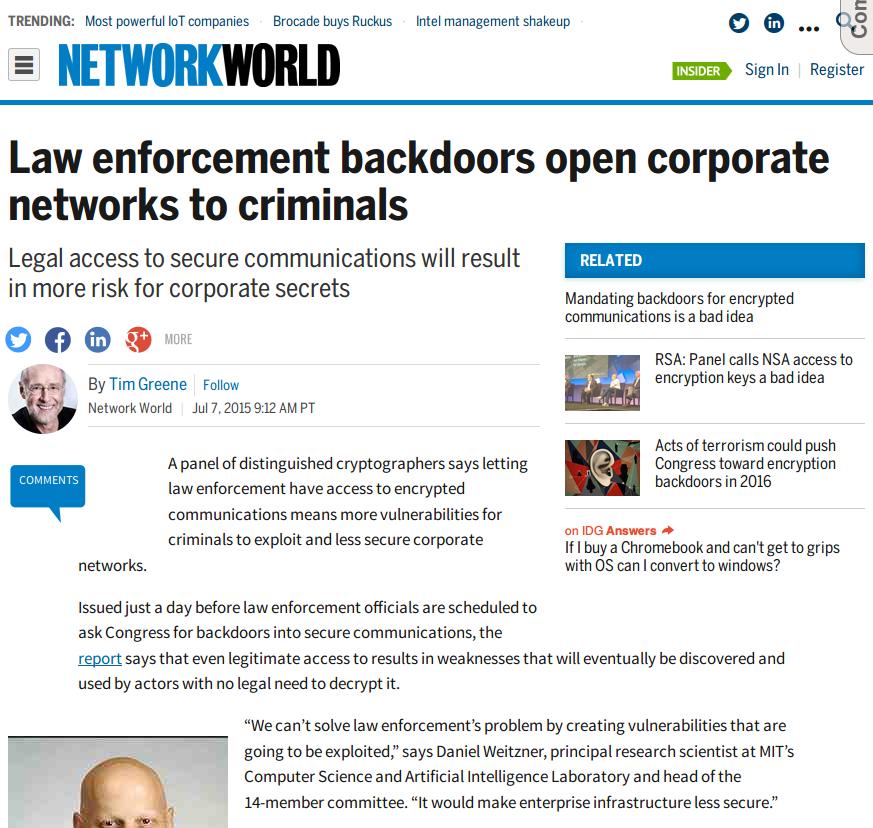
\includegraphics[scale=0.28]{backdoor_criminals.png}
%http://www.networkworld.com/article/2944866/security0/law-enforcement-backdoors-open-corporate-networks-to-criminals.html
% the thing with backdoors is that they will be found and used also by criminals
\end{frame}

\begin{frame}{Compromised build environment}
Unlikely but very serious\\
The build host is the one component you still have to trust with traditional open source distributions. % so far
\\[0.2cm]
\emph{Problems:}
\begin{itemize}
\item Hard to detect
\item Once infected, almost impossible to clean
\item Can result from any backdoored software with enough access
\end{itemize}
\\[0.2cm]
\pause
\emph{What can we do to prevent?}
\begin{itemize}
\item Tight access control and monitoring
\item Redundant build environments  % usually not binary equal. Even timestamps can make the difference
\item Debian reproducible builds    % closing the last loophole
\end{itemize}
\end{frame}

\begin{frame}{Debian reproducible builds}
%ToDo : add content
\end{frame}

\begin{frame}{Compromised build tools}
\emph{Unlikely but very serious}
\\[0.2cm]
\begin{itemize}
\item Not much you can do
\item Trust hwomever sold it to you
\item Use a well reviewed open source tool chain
\end{itemize}
% hard to defend against
\end{frame}

\begin{frame}{Bundling malware by publisher}
\emph{Examples:}
\begin{itemize}
\item Oracle Java
\item Compression tool served by Npackd % a package manager for windows
\end{itemize}
\\[0.2cm]
\pause
\emph{As a software publisher:}
\begin{itemize}
\item Just don't do it!
\item Loosing users and trust is not worth the few bucks
\end{itemize}
\\[0.2cm]
\pause
\emph{As the user:}
\begin{itemize}
\item I try not to use software if I have reason to beleve it is compromised % even if it is forced on us
\item There are always plenty of good alternatives
\end{itemize}
\end{frame}

\begin{frame}{Insecure coding practices}
\emph{As a software publisher:}
\begin{itemize}
\item I won't go into details here
\item Events just like today address this very issue
\end{itemize}
\\[0.2cm]
\pause
\emph{As the user:}
\begin{itemize}
\item With closed source software, you can only guess
\item A shiny GUI tells nothing about what's behind
\item If it crashes a lot, there might be more at odds
\end{itemize}
\end{frame}

\begin{frame}{Bribed timestamping provider}
This is probably the least severe case here, but still not wanted.
\\[0.2cm]
\begin{itemize}
\item Proof of existence can be a hash of a document published in a newspaper
\item There is a service called proof of existence that stores the hash on the BitCoin blockchain
\end{itemize}
\end{frame}

\begin{frame}{Compromised certificate authority}
%ToDo : add content
\end{frame}

\begin{frame}{NameCoin}
%ToDo : add content
\end{frame}

\begin{frame}{Private key stolen or unintentionally published}
\begin{itemize}
\item A surprising number of private keys were found in github repositories
\item Never send a private key over unencrypted eMail % Reto has a story to this
\item Never store a private key unencrypted on a cloud starage
\item If possible store private keys only on airgapped machines and hardware devices
\item A good example is the YubiKey NEO with an OpenPGP applet
\item If you have to store it on disk, restric the access rights
\end{itemize}
\end{frame}


\end{document}

